\setlength{\parindent}{0pt}

\clearpage
\section{Liveness Analysis}
(Prepared by Jai Arora)
\vspace{0.3cm}

Previously, we saw a type of Global Optimisation called Global Constant Propagation, which required the knowledge of the whole program.
After all the constants have been propagated globally, there can be a scope for eliminating dead code.

\begin{figure}[H]
    \centering
    
\includegraphics[height=6cm]{images/Module81_1.png}
    \caption{Motivation for Liveness Analysis}
\end{figure}

Consider a statement $x := ...$\\
Questions to ask: Is $x$ live or dead just after the statement? What does liveness mean?\\
Ans: A variable $x$ is live after a statement if it can be used in the downflow logic\\

Consider the following example:
\begin{figure}[H]
    \centering
    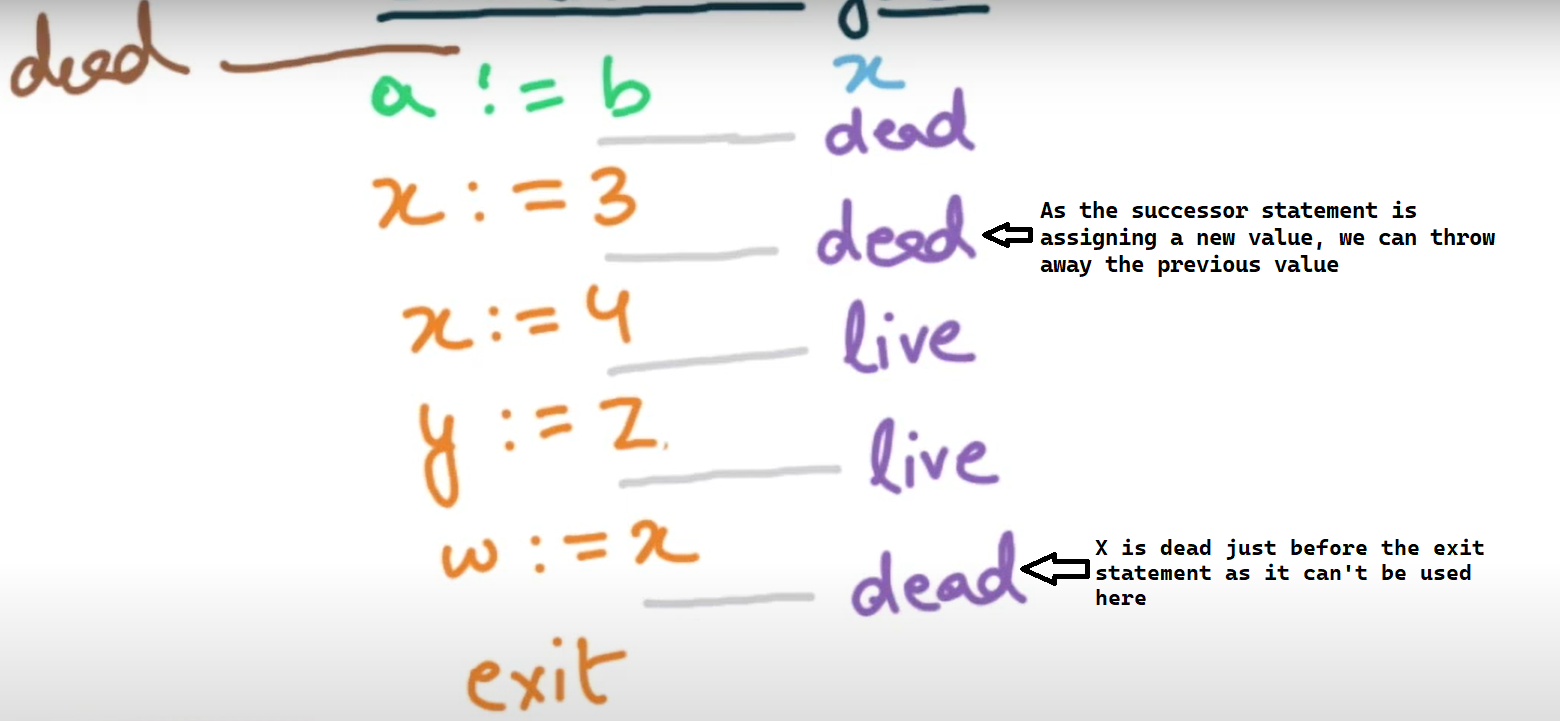
\includegraphics[height=6cm]{images/Module81_2.png}
    %\caption{Converting to SSA Example}
\end{figure}

\vspace{0.3cm}
The above intuition can be formalized as follows. A variable $x$ is live at a statement $s$ if:
\begin{itemize}
    \item There exists a statement $s'$ that uses $x$
    
    Eg:- $s':$ $y := f(...,x,...)$
    \item There is a path from $s$ to $s'$ (directed)
    \item The path has \underline{no intervening assignments} to $x$
\end{itemize}

Once we have figured out if a variable $x$ live or dead at all statements, then we can easily identify dead code.\\
A statement $x := ...$ is dead code if $x$ is dead immediately after the assignment.
In this case, as the variable is not being used in the downflow logic, which means that we can simply remove the assignment.

\subsection{Liveness Analysis as a DFA}
In this analysis, the property that we want to know at a particular program point is the liveness of a particular variable. In the example above, we found the liveness value at one point using the other values.
This gives us an intuition for a $\textbf{Transfer Function}$, and hence we use a DFA for this problem as follows:
\begin{itemize}
    \item Express liveness at a program point based on the liveness of the successor program point (Backward Dataflow)
    \item The Liveness property for a variable $x$ would take a boolean value
    
    \hspace*{0.1 in}${\tt true} \rightarrow$ The variable may be live (This is a conservative value)\\ 
    \hspace*{0.1 in}${\tt false} \rightarrow$ The variable is definitely dead (not live)
\end{itemize}

\subsection{Ordering of Liveness Values}
As seen previously, it really helps to construct a partial ordering because it makes the rules concise. So we do would the same here. Define the ordering as:

\begin{center}
    ${\tt true} \leqslant {\tt false}$
\end{center}
\begin{figure}[H]
    \centering
    
\includegraphics[height=2cm]{images/Module81_3.png}
    \caption{The Semilattice of Liveness Values}
\end{figure}

Once this ordering has been established, it can be easily seen that the greatest lower bound of any $2$ values $x, y$ would be the boolean OR of those values.
$$glb(x,y) = x \vee y$$
$$glb(x_1,x_2,...,x_n) = x_1 \vee x_2 \vee ... \vee x_n$$

